\documentclass[aspectratio=169]{beamer}
\usepackage{amssymb,amsmath}
\usepackage{graphicx}
\usepackage{url}
\usepackage{color}
\usepackage{pagenote}[continuous,page]
\usepackage{cancel}   % Math "cancelto"
\usepackage{relsize}	% For \smaller
\usepackage{url}			% For \url
\usepackage{epstopdf}	% Included EPS files automatically converted to PDF to include with pdflatex

%For MindMaps
\usepackage{tikz}%
\usetikzlibrary{mindmap,trees,arrows}%

%%% Color Definitions %%%%%%%%%%%%%%%%%%%%%%%%%%%%%%%%%%%%%%%%%%%%%%%%%%%%%%%%%
%\definecolor{bordercol}{RGB}{40,40,40}
%\definecolor{headercol1}{RGB}{186,215,230}
%\definecolor{headercol2}{RGB}{80,80,80}
%\definecolor{headerfontcol}{RGB}{0,0,0}
%\definecolor{boxcolor}{RGB}{186,215,230}

%%% Save space in lists. Use this after the opening of the list %%%%%%%%%%%%%%%%
%\newcommand{\compresslist}{
%	\setlength{\itemsep}{1pt}
%	\setlength{\parskip}{0pt}
%	\setlength{\parsep}{0pt}
%}

%\setbeameroption{show notes on top}

% You should run 'pdflatex' TWICE, because of TOC issues.

% Rename this file.  A common temptation for first-time slide makers
% is to name it something like ``my_talk.tex'' or
% ``john_doe_talk.tex'' or even ``discrete_math_seminar_talk.tex''.
% You really won't like any of these titles the second time you give a
% talk.  Try naming your tex file something more descriptive, like
% ``riemann_hypothesis_short_proof_talk.tex''.  Even better (in case
% you recycle 99% of a talk, but still want to change a little, and
% retain copies of each), how about
% ``riemann_hypothesis_short_proof_MIT-Colloquium.2000-01-01.tex''?

\mode<presentation>
{
  \usetheme{CambridgeUS}
  \usecolortheme{dolphin}
  \useoutertheme{default}
  \useinnertheme{default}
  \setbeamercovered{invisible} % or whatever (possibly just delete it)
}
\beamertemplatenavigationsymbolsempty

\usepackage[english]{babel}
%\usepackage[latin1]{inputenc}
\usepackage{subfigure}

\usepackage{times}
\usepackage[T1]{fontenc}
\usepackage{CJKutf8}

%% makes the ppagenote command for figure references at the end.
\makepagenote
\renewcommand{\notenumintext}[1]{}
\newcommand{\ppagenote}[1]{\pagenote[Page \insertframenumber]{#1}}

\title[Experiment Design (01CH740)]{Experiment Design for Computer Sciences (01CH740)}
\author[Claus Aranha]{Claus Aranha\\{\footnotesize caranha@cs.tsukuba.ac.jp}}
\institute[U. Tsukuba]{University of Tsukuba, Department of Computer Sciences}


\subtitle[Intro]{Topic 00 - Course Introduction}
\date{2023/04/14}

\begin{document}
\begin{CJK}{UTF8}{ipxm}

\begin{frame}
  \maketitle

  \vfill

  \hfill Version 2023.1
\end{frame}

\section{Course Motivation}

\begin{frame}
  \begin{center}
    Part I -- What is this course about?
  \end{center}
\end{frame}

\begin{frame}{What is this course about?}

  \begin{block}{From the syllabus}
    \emph{The collection and analysis of data through experiments is
      one of the cornerstones of the scientific method. In this
      course, we study the general philosophy and methods behind
      experimentalism: Why do we perform experiments, what is a
      good/rigorous experiment, how to plan and design a rigorous
      experiment, and how to perform statistical analysis on
      experimental data.}
  \end{block}
  \bigskip

  What does this mean?
\end{frame}

\begin{frame}{What is this course about?}{}

  The key idea of this course is to learn \structure{how to do an
    experiment in a systematic manner}.\bigskip

  \begin{center}
    \includegraphics[width=.6\textwidth]{../img/irasutoya_pdca}\ppagenote{PDCA flowchart from \url{https://www.irasutoya.com}}
  \end{center}\bigskip

  i.e., "how to apply the PDCA cycle for science?"
\end{frame}

\begin{frame}{Why is this course necessary?}{Frequent errors when designing an experiment}

  There are some errors that are often found in CS experiments:
  \bigskip

  \begin{itemize}
    \item The experiment does control for noise;\\
      \structure{Problem: Is the result just a coincidence?}
    \item The experiment does unfair comparisons between methods;\\
      \structure{Problem: Is the result valid in the general case?}
    \item The experiment is not clear / not reproducible;\\
      \structure{Problem: Can this experiment help other people?}
    \item etc...
  \end{itemize}\bigskip

  Many of these errors happen because of experiments done
  carelessly. So let's learn to think more carefully about them!


\end{frame}

\begin{frame}{Why is this course necessary?}{The "Invisible
    Curriculum" -- things that are not taught in classes}

  The \structure{Invisible Curriculum} are things that are necessary
  for your work as an academic, but that you usually can't learn in a
  lecture, and must discover by \alert{trial and error}. For
  example:\bigskip

  \begin{columns}
    \column{0.7\textwidth}
    \begin{itemize}
      \item How do I prepare an experiment?
      \item When do I publish a result?
      \item How do I review a paper?
      \item How do I teach a lecture?
      \item What are grants?
      \item ...
    \end{itemize}\bigskip

    The goal of this course is to shed light in one of these points:\\
    \emph{What is an experiment, and how do I prepare it?}

    \column{0.3\textwidth}
    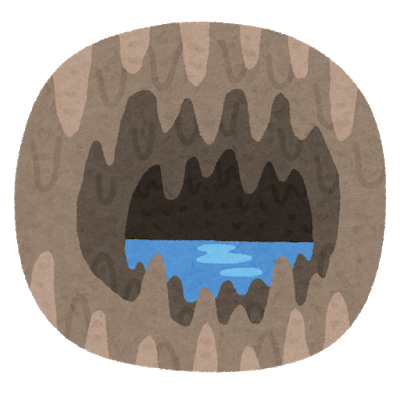
\includegraphics[width=1\textwidth]{../img/irasutoya_cave}\ppagenote{Cave illustration from \url{https://www.irasutoya.com}}
  \end{columns}
  \bigskip

\end{frame}

\section{Course Topics}
\begin{frame}{Course Topics}
  The main things that you will learn in this course are:\bigskip

  \begin{itemize}
    \item What is an experiment:
    \begin{itemize}
      \item What is the role of an experiment in Science?
      \item How do I design an experiment to answer a scientific question?
      \item What are the characteristics of a \structure{good} experiment?
      \item How do I analyse the results of an experiment?
    \end{itemize}\bigskip

    \item Statistical tools for analyzing experimental data:
    \begin{itemize}
      \item Basic statistics for data analysis and visualization;
      \item Statistical Inference ("Statistically Significant Results");
      \item Statistical testing for single, paired, and multiple sample testing;
      \item How to calculate the sample size and power of an experiment;
    \end{itemize}
  \end{itemize}
\end{frame}

\begin{frame}{Course Topics}{Limitations: This is only an introductory course!}

  \begin{columns}
    \column{0.8\textwidth}
    This course is an \structure{introduction} to design of
    experiment. My main objective is to teach you {\bf why} designing
    experiments is important, and what problems can happen when you
    don't do this. Not to teach all the statistical tests.
    %\column{0.1\textwidth}
    \column{0.2\textwidth}
      \includegraphics[width=1\textwidth]{../img/irasuto_sprout}
      \ppagenote{Sprout image from \url{https://www.irasutoya.com}}
  \end{columns}
  \vfill

  Each experiment, in each research, will require a different way of
  doing statistical analysis. Also, some advanced topics (bayesian
  statistical analysis) will not be covered here. I hope that after
  this course you will have a solid understanding of the concepts to
  read and learn the advanced tests required of your own research.
\end{frame}

\begin{frame}
  \begin{center}
    Part II -- Practical Details
  \end{center}
\end{frame}

\section{Practical Details}
\begin{frame}
  \frametitle{Practical Details about the course}
  \begin{itemize}
    \item Class Format;
    \item Communication Channels;
    \item Course Materials;
    \item Course Schedule;
    \item Grading;
    \item Other topics;
  \end{itemize}\vfill

  \alert{Note}: The latest and most correct information about course policy is always on manaba.
\end{frame}

\subsection{Course Format}
\begin{frame}[t]{Class Format -- In person (Online Support)}
  \begin{itemize}
  \item The lectures will be in person.
    \begin{itemize}
    \item The class materials do not fill the entire 150 minute period (about 1 hour material).
    \item I like to ask plenty of questions, and hold discussions during class.
    \item Also, breaks when necessary.
    \end{itemize}
  \item Final exam will be in person too.
  \item If you cannot come to class, videos from last year will be available.
    \begin{itemize}
    \item In that case, please ask questions on manaba!
    \end{itemize}
  \end{itemize}
\end{frame}

% \subsection{Course Format}
% \begin{frame}{Class Format -- Online, On demand}
%   \begin{itemize}
%   \item We have students in several time zones, so I will teach you
%     using pre-recorded videos and lecture materials.
%     \begin{itemize}
%       \item Please watch the videos in full, at a time and speed of your convenience. Videos are published on Youtube and Teams.
%     \end{itemize}
%     \item On Fridays, 15:15-18:00 JST, I will hold "office hours" to answer questions about the class and anything else.
%     \begin{itemize}
%       \item I will not count attendance on office hours. Come if you have questions.
%       \item I will be online on TEAMS, and you can also come to my office if you want (SB904).
%       \item Please send a message if you come to my office.
%       \item If you cannot come to the office hours, please see the next slide.
%     \end{itemize}
%     \item \alert{Exception: The final exam is Online Syncronous. If this is too difficult for your timezone, please talk to me.}
%   \end{itemize}

% \end{frame}

\begin{frame}[t]{Communication Channels}{}
  Communication between us is very important. Do not leave questions unanswered!\bigskip

  Communication channels by priority:
  \begin{enumerate}
  \item Ask questions during the class. The material does not cover
    the full class time, so you can stop and ask if anything is not
    clear.
  \item Use the manaba forums to ask questions outside of class
    hours. By opening a forum thread, other students with similar
    questions can also see the answer.
  \item Feel free to e-mail me if you have questions that can not be
    shared with other students.
  \end{enumerate}\bigskip

  Also, every lecture I post an {\bf Attendance Survey} on manaba. The
  survey is not graded, but \alert{you must take the survey to count
    for attendance!}
\end{frame}

\subsection{Course Materials}
\begin{frame}[t]{Course Materials}
  \begin{itemize}
  \item The lecture notes are published in the "manaba" system.
  \item Access code for 2023: \alert{9352484}. Use this code if you can't access manaba yet.
    \bigskip

  \item The course materials are also available on github:\\
    \url{https://caranha.github.io/ExperimentDesignCS/}.\medskip

  \item This year, the course is fully in person. I strongly recommend
    that you come to class. However, the videos from 2022 will be
    listed on Manaba if you need to miss a lecture.
    \begin{itemize}
    \item Please note that there may be new material not covered in the videos.
    \end{itemize}
  \end{itemize}
\end{frame}

\begin{frame}{Course Materials}{Acknowledgements}
  \begin{columns}
    \column{0.8\textwidth}
    The lecture notes were produced based on the "Design and Analysis of Experiments" material produced by Felipe Campelo. You can reach the original lecture notes on: \url{https://github.com/fcampelo/Design-and-Analysis-of-Experiments}

    \column{0.2\textwidth}
    \hfill\includegraphics[width=1\textwidth]{../img/Felipe_Campelo}
  \end{columns}
  \bigskip

  All good ideas are thanks to Felipe (and other contributors) all errors are my own :-) (Please submit errors as github issues!)
\end{frame}

\begin{frame}[t]{Course Materials}{Books and Links}
  \begin{itemize}
  \item The list of books, papers, and webpages used to assemble this course
    is listed on manaba and on github.
  \item Please do extra reading. It is not possible to cover all
    topics related to experiment design in just one semester.
  \end{itemize}
\end{frame}



\subsection{Course Schedule}
\begin{frame}{Course Schedule}{}
  \begin{itemize}
    \item 4/14 Topic 01 -- Course Introduction, What is Experimentation
    \item 4/21 Topic 02 -- Point and Interval Indicators
    \item 4/28 Topic 03 -- Inference Testing I
    \item 5/05 (Golden Week, no Class)
    \item 5/12 Review -- Class Review and Discussion of Report I
    \item 5/19 Topic 04 -- Inference Testing II
    \item 5/26 Topic 05 -- Inference Testing III
    \item 6/02 Topic 06 -- Sample Size and Experiment Power
    \item 6/09 Topic 07 -- Block and Factorial Designs I
    \item 6/16 Topic 08 -- Block and Factorial Designs II
    \item 6/23 Review -- Class Review and Consultation about Report II
    \item 6/30 Final Exam
\end{itemize}
\end{frame}

%## Report 1 -- Simple Experiment
%- 04/20 Experiment Topic Submission
%- 05/09 Experiment Report Submission

%## Report 2 -- Experiment Analysis
%- 05/23 Experiment 2 Topic Submission
%- 06/18 Experiment 2 Presentation
%- 07/02 Experiment 2 Report Submission

\subsection{Grading}
\begin{frame}{Grading}
  Two reports (R1, R2), and a final examination (E). Each graded from 0 to 100.
  The final Grade (FG) is:

  \begin{equation*}
    FG = 0.2*R1 + 0.4*R2 + 0.4*E
  \end{equation*}
  \bigskip

  The letter grade for this course follows the Tsukuba standard ($< 60: D; < 70: C, < 80: B, < 90: A$)
\end{frame}

\begin{frame}{Grading}{Final Examination}
  \begin{itemize}
    \item Covers the topics of the entire course.
    \item Must be answered in English.
    \item You may prepare {\bf one A4 page of handwritten notes (both sides)}, and use it on the test.
    \begin{itemize}
      \item The notes have no fixed format, and can be in any language.
      \item The notes must include your name and student ID, and must be turned in with the exam. The notes will not be graded.
    \end{itemize}
    \item You can bring a dictionary to the exam.
    \item No other consultation is allowed in the exam.
  \end{itemize}
\end{frame}

\begin{frame}{Grading}{Reports}
  Two "mini-papers". The student must plan, perform, and analyze an experiment of their own choice:\bigskip

  \begin{itemize}
    \item Choose a scientific question to answer
    \item Design an Experiment to gather data to answer that question
    \item Execute the experiment, following the design
    \item Analyze the data, following the design
    \item Make a conclusion, based on the analysis of the data
  \end{itemize}\bigskip

  The different between report 1 and report 2 are the expectations.\\ Please see details in manaba.
\end{frame}

\section{Others}
% \begin{frame}{Other Topics:}{Computer Science English Program (CSE)}
%   The CSE supports a master degree fully in English. If you plan to take most of your classes in Enslish, do not forget to enroll in the CSE:
%   \bigskip

%   Send an e-mail to \structure{s-g30@cs.tsukuba.ac.jp} with this info:
%   \begin{itemize}
%     \item Your name (ASCII and Kanji)
%     \item Student ID
%   \end{itemize}\bigskip


%   For more information, see the orientation material at the "New Student Orientation" course on manaba.
% \end{frame}

\begin{frame}{Other Topics:}{Self Introduction}
  \begin{columns}
    \column{0.4\textwidth}
    \includegraphics[height=.8\textheight]{../img/pinhole}
    \column{0.6\textwidth}
    {\small
    \begin{itemize}
      \item \structure{Name:} Claus Aranha;
      \item \structure{Country:} Brazil;
      \item \structure{Research Topics:}
      \begin{itemize}
        \item Evolutionary Algorithms;
        \item Artificial Life;
      \end{itemize}
      \item \structure{Hobbies:}
      \begin{itemize}
        \item Game Programming;
        \item Geocaching;
      \end{itemize}
        \smallskip

      \item \structure{webpage:}\\
      {\smaller \url{http://conclave.cs.tsukuba.ac.jp}}
      \medskip

      Ask me anything you want!
    \end{itemize}
    }
  \end{columns}
\end{frame}

\begin{frame}{}
  \begin{center}
    Part III - Report I
  \end{center}
\end{frame}

\begin{frame}{Report I}{General Information}
  Write a "mini paper" about an experiment that you choose, prepare, execute and analyze. Specifically, you must:\medskip

  \begin{itemize}
    \item Choose a question to investigate using a scientific experiment.
    \item Design the experiment (choose variables, data collection and analysis protocol)
    \item Execute the experiment following the data collection protocol.
    \item Analyze the data obtained following the data analysis protocol.
    \item Take note of any surprising or unsurprising findings, and prepare a conclusion for the experiment.
  \end{itemize}\medskip

  The report must summarize the above points (the question, experiment designs, data collection, data analysis, and conclusion).
\end{frame}

\begin{frame}{Report I}{Expectations}
  In the first report, you should select a simple experiment with a single dependent variable and a single independent variable, and calculate simple statistical intervals of values observed for the dependent variable. These topics are covered in lectures 1 and 2.\smallskip

  The report will be graded by:
  \begin{itemize}
    \item Whether it describes a coherent scientific experiment to answer the chosen question;
    \item The quality of the data analysis;
    \item The quality of the result presentation and discussion;
  \end{itemize}\bigskip

\alert{Note that you are NOT expected to use the null-hypothesis model in this report (lectures 4-6). Doing the test wrongly may deduct points.}
\end{frame}



\begin{frame}{Report I}{How to choose an experiment topic}
  \begin{itemize}
    \item If possible, choose something from your own research;
    \medskip

    \item Experiments from your day to day life are also good;
    \begin{itemize}
      \item Comparing cooking techniques is always fun;
      \item When collecting data, be careful of measuring errors;
    \end{itemize}
    \medskip

    \item When in doubt, comparing algorithms is an easy choice;
    \begin{itemize}
      \item Make sure to choose an appropriate metric to report!
    \end{itemize}
    \medskip

    \item Make sure you choose an experiment that you can perform!
    \bigskip

    \item This article might be insightful: \url{https://williamghunter.net/articles/101-ways-to-design-an-experiment}
  \end{itemize}
\end{frame}

\begin{frame}[t]{Report 1}{Rules and Deadlines}
  \begin{itemize}
    \item {\bf Report Deadline: 05/01, 23:00} -- submit on manaba\bigskip

    \item The report must be in English.\bigskip

    \item Submit the report as a PDF file, don't forget your name/ID.
    \item Submit also a ZIP file with all the data/scripts necessary to reproduce your analysis.
    \bigskip

  \item \alert{Aspiring scientists should be specially wary of
      plagiarism. Please see manaba for details.}
  \end{itemize}

\end{frame}


\section{Backmatter}
\begin{frame}{About these Slides}
  These slides were made by Claus Aranha, 2022. You are welcome to copy, re-use and modify this material.
  \bigskip

  These slides are a modification of "Design and Analysis of Experiments (2018)" by Felipe Campelo, used with permission.
  \bigskip

  Individual images in some slides might have been made by other
  authors. Please see the following references for those cases.
\end{frame}

\begin{frame}[allowframebreaks]{Image Credits}
  \printnotes
\end{frame}

\end{CJK}
\end{document}
